\section{Type of communication}
Communication is highly important in our lives, especially in any system. The meaning behind communication network is a pattern or shape that is used in an organization to efficiently transmit information. The communication network is the established system in which messages can travel in one or more ways inside the company depending on the requirements. There are two kinds of communication. Wireless communication is the first, while wired communication is the second. For further information, multiple communication networks may be built based on their efficacy depending on the system's needs. 

\subsection{wireless network}
Wireless means that there is no physical touch between two sites. Thus, wireless networks are computer networks that are not connected by any form of cable. The deployment of a wireless network allows businesses to avoid the costly procedure of installing wires in buildings or connecting multiple equipment locations. Radio waves serve as the foundation of wireless systems, acting as a mode of transport for data transmission and reception. The examples of wireless networks are shown below.
\subsubsection{Bluetooth}
Bluetooth was developed as an alternative to using cables and wires to build a network. It was designed to unite telecommunications protocols under a single worldwide standard. It is used for wireless communications and broadcasts over short distances. Bluetooth-enabled devices construct ad hoc networks (networks with a single function) with one another to exchange or broadcast data. While Bluetooth was designed to be a cable replacement, it is now extensively utilized because it generates a dynamic Personal Area Network (PAN) \cite{b2}.

\subsubsection{Wi-Fi}
Wi-Fi is a wireless networking protocol. Wi-Fi is simply a very modern digital radio that operates at frequencies in the electromagnetic spectrum ranging from 2 gigahertz to 5 gigahertz, which is roughly the same as microwave ovens. Each standard is an approved modification throughout time. The standards operate at variable frequencies, provide varying bandwidth, and support varying numbers of channels \cite{b3}.

\subsection{Wired network}
A wired network is one of the most popular types of wired arrangement. Ethernet cables are commonly used in wired networks to transport data between linked PCs. A single router may connect all PCs in a small wired network. Larger networks frequently have many routers or switches that communicate with one another. One of these devices is often linked to a cable modem, T1 line, or other sort of Internet connection, which offers Internet access to all network devices. Wired can also refer to peripheral devices. Below are the example of wired network.

\subsubsection{UART}
In UART communication, two UARTs communicate directly with each other. The transmitting UART turns parallel data from a controlling device, such as a CPU, into serial data and transmits it to the receiving UART, which converts the serial data back into parallel data for the receiving device. Only two wires are necessary to transfer data between two UARTs. Data is sent from the Tx pin of the transmitting UART to the Rx pin of the receiving UART. The diagram below depicts the UART connection \cite{b4}.

\begin{figure}[h]
    \centering
    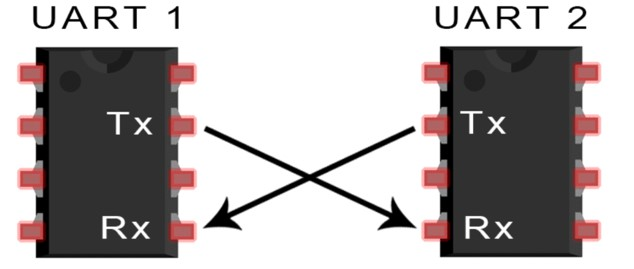
\includegraphics[width=0.5\textwidth]{UART}
    \caption{Connection of UART}
    \label{fig:UART}
\end{figure}

\subsubsection{I2C}
I2C combines the greatest qualities of SPI and UARTs. I2C allows you to connect several slaves to a single master (similar to SPI) and control single or multiple slaves. This is especially useful when many microcontrollers are recording data to a single memory card or displaying text on a single LCD. I2C communication, like UART communication, uses just two wires to send and receive data between devices: Because I2C is synchronous, a clock signal shared by the master and slave syncs the bit output to the bit sampling. The clock signal is always in the hands of the master. SDA (Serial Data) - The data transmission and reception line between the master and slave. Serial Clock Line (SCL) — The line that carries the clock signal \cite{b4}.

\begin{figure}[h]
    \centering
    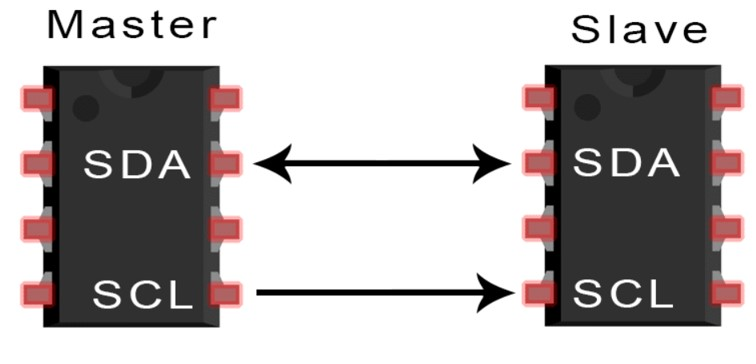
\includegraphics[width=0.5\textwidth]{I2C}
    \caption{Connection of I2C}
    \label{fig:I2C}
\end{figure}

